\section{LITERATURE REVIEW} \label{chap:literature_review}
The security of an application showed its first impacts around the beginning of the century with the increasing popularity of the \acrfull{www} and the enablement of user-fuelled websites (like social media). This rapid evolution paired with the common lack of knowledge of the users but also of the developers caused the birth of Denial of Service and Cross-Site Scripting attacks among others \cite{Hoffman2024}.

\subsection{Application Security Testing}
\acrfull{ast} includes every procedure that evaluates software security, these methods may include manual or automatic testing; manual testing may perform in the form of penetration tests, but automatic testing has 2 common variants, static (\acrshort{sast}) and dynamic (\acrshort{dast}).

\acrlong{sast} is a white-box approach to software security where we have access to source code and through analysis a developer can attempt to find vulnerabilities in it; its practice is also commonly described as finding code errors. 

\acrlong{dast} is on the other hand also known as the black-box approach -- it has no knowledge of how a software is coded or designed. It only knows how to interact with the software and attempts to do so in a manner that it can find malfunctions and failures in the program execution; its results are the inputs used to break the application flow.

There is also a practice known as \acrlong{iast} which despite being described as a white-box technique, it also examines the software security during runtime, and it must be integrated with it. However, this represents runtime overhead and inability to detect client-side vulnerabilities \cite{sast-dast-iast}.

\subsubsection{SAST vs. DAST}

After looking at the research performed by \cite{SASTvsDAST}, a summarized version of the comparison between the two methods can be described as seen in \Cref{tab:sast_vs_dast}.

\begin{table}[ht]
\centering

\begin{tabular}{cc}
\textbf{\acrshort{sast}} & \textbf{\acrshort{dast}}\\
\hline
White-box testing  & Black-box testing \\
Test from the inside out  & Test from the outside in \\
Test internal behaviour  & Test external expectations \\
Validate code quality  & Validate system functionality \\
High granularity  & Low granularity \\
Full knowledge of application structure & No knowledge of application structure \\

\end{tabular}
\caption{Summarized Theoretical Comparison of \acrshort{sast} \& \acrshort{dast}}
\label{tab:sast_vs_dast}
\end{table}

This theoretical comparison is presented with a more practical one, where \cite{SASTvsDAST} tests, analyses, and studies different scans with different tools for both methods. The metrics used are the standard True Positive, True Negative, False Positive, False Negative (TP, TN, FP, FN) and are required to calculate the True Positive Rate (TPR) and False Positive Rate (FPR) which happen to be the most relevant rates that contribute to a grade of accuracy and confidence in each cybersecurity tool used. One such way to infer an accuracy metric is using Youden's Index that can be seen in \cref{equ:youden_index} as \citeauthor{owasp_youden_index} \cite{owasp_youden_index} described for the OWASP Benchmark.

\begin{mycapequ}[htbp]
    \centering
    \caption{Youden's Index or Youden's J statistic}
    \begin{equation}
        Youden index (Score) = TPR (True Positive Rate) - FPR (False Positive Rate)
    \label{equ:youden_index}
    \end{equation}
\end{mycapequ}


\citeauthor{owasp-devsecops-dast} \cite{owasp-devsecops-dast} also describes \acrshort{dast} as ``especially helpful for detecting: input or output validation, authentication issues, server configuration mistakes'' and specifies that they ``allow for sophisticated scans on the client side and server side'' and require no implementation information (source code, framework, etc.). 

\subsubsection{Software Development Life Cycle}

An analysis of software security necessarily encompasses the entire development lifecycle, with particular emphasis on testing and deployment. Integrating specialized security testing within the validation phase is essential; however, the deployment phase remains equally critical, as it represents a high-risk transition point within the system's lifecycle \cite{SDLC}. Moreover, it is worth noting how the cost of remediating a risk increases the further down the life cycle it is detected and flagged when compared to those found earlier \cite{SAST_opensource}.

After a careful analysis of the two techniques to test application security, and a quick glance at \Cref{fig:SDLC}, what makes most sense for most organizations is to execute static security scans as part of the testing phase. If a more complete deployment is required for dynamic tests, then we could be looking at a later stage: deployment. This also depends greatly on how companies implement CI/CD; if they do it well enough, then the testing phase just became much more agile and dynamic, making it possible to secure software statically directly in the implementation phase and dynamically in the testing phase, detecting problems much earlier and reducing costs in overall risk management \cite{SASTvsDAST,Rangnau2020}.
\begin{figure}[ht]
    \centering
    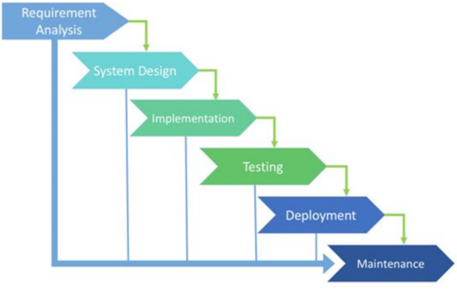
\includegraphics{images/sdlc.png}
    \caption{Software Development Life Cycle Model \cite{SDLC}}
    \label{fig:SDLC}
\end{figure}

\subsection{SAST - Static Application Security Testing}
Expanding on the white-box technique, most vulnerabilities are due to developer's lack of awareness and/or bad programming practices \cite{SAST_opensource} in such a way that \citeauthor{owasp-devsecops-sast} \cite{owasp-devsecops-sast} defines it ``as part of a Code Review'', a ``method of computer program debugging that is done by examining the code without executing the program'', and also a good technic to help find:
    \begin{itemize}
        \item ``Syntax violations''
        \item ``Security vulnerabilities''
        \item ``Programming errors''
        \item ``Coding standard violations''
        \item ``Undefined values''
    \end{itemize}

\subsubsection{Symbolic Execution}
Inside \acrshort{sast}'s set of technics, introduced by \cite{King1976}, we find symbolic execution engines which can help protect systems that range from modern \acrfull{soc} designs and hardware Trojans \cite{Vafaei2021}, to binary-level security analysis such as malware comprehension \cite{David2016} and even a symbiosis between symbolic and concrete execution \cite{Gritti2020}.
All these tools share a common requirement: any instruction set ranging between machine code to source code. These tools excel by mimicking the execution of the analysed software, controlling each value the input influences in the form of symbolic values or variables.

However, a more in-depth look at symbolic execution unveils some obstacles, such as path explosion, constraint solving, environment modelling and others. These symbolic values are allowed to be anything at a first stage, and its value is deciphered further down in the execution path, reducing the possibilities at every branch the execution encounters. The branching happens after performing constraint solving, a very time expensive operation especially when the tested source is of high complexity \cite{Zhang2022}. 

Constraint solving occurs at every moment where a variable value impacts the flow of execution or even once a symbolic variable takes part in any arithmetic computation. This escalates once these computations become of a non-linear nature, such as non-linear expressions and non-linear floating-point computations \cite{Kroening2008}.

Path explosion is one concern found in many high performance problems: the input is sufficiently complex for any sort of resource - be it time, memory, or even processing capacity - to escalate tremendously and becoming unreasonable in a standard environment. When it comes to symbolic execution, a new path is encountered every time a constraint is solved; from that point on, that constraint is a path condition. To better understand this concept, here's an example using the tool \textit{KLEE} according to \cite[p. 3]{Cadar2008}: 
\begin{quote}
``When KLEE detects an error or when a path reaches an exit call, KLEE solves the current path's constraints (called its path condition) to produce a test case that will follow the same path when rerun on an unmodified version of the checked program (e.g., compiled with gcc).''
\end{quote}

Environment modelling is another very common problem in software analysis techniques given how much software development relies on third-party libraries today. This problem escalates whenever these dependencies are packaged as binaries, or the sources are `super-optimized', the paths exploration and consequently the constraint solving may fail which may result in false positives or false negatives \cite{Cadar2008}.
\vfill

\subsection{DAST - Dynamic Application Security Testing} 

The black-box method of testing is very tightly coupled with a hacker perspective of the application; the intention is to find design and/or implementation flaws that cause the system to break down or allow its security to be compromised. Sometimes, to be able to do this a better understanding of the code is required and the testers will frequently find themselves trying to understand how the application is coded.
This technique is known for its low false positive rates, its language independent nature and its ability to detect configuration related attacks. The abstraction of the software implementation is possible because \acrshort{dast} tools require a runtime test case, this means that in the \gls{sdlc} this is applied in the later stages (shift-right) \cite{DAST_description}.

\subsubsection{Fuzzing}
One way to dynamically test software is through fuzzing techniques; this consists of feeding random input with the objective of breaking the application logic or even its execution. \cite{Godefroid2020} also describes it as ``test generation and execution with the goal of finding security vulnerabilities''. Although \textit{fuzzing} is a quick technique, it generally has poor path coverage on its own.

\subsubsection{Dynamic Taint Analysis}
\cite{Schwartz2010} explain that dynamic taint analysis also operates in running programs, but this time by carefully analysing application inputs and each operation to keep track of new and derived taint in an attempt to prevent execution of potentially harmful instructions. Usually, a tainted variable is influenced by user input and then every other variable that is influenced by the first. This technique can be summarized in three steps or \textit{taint policies}: taint introduction, propagation, and checking.

All variables are considered untainted and that only changes when raw user input is stored in one of them, then it becomes a tainted variable. Following user input comes application logic, the same logic that through expressions will contaminate any other variable that interacts with the first set that was tainted by user input. However, once the application gets to a critical operation, it can decide on performing it or not based on how tainted critical variables are  (taint checking).

\subsection{Symbolic Execution}

This work is focused on the static method of application security testing, symbolic execution, and as such we will analyse some available tools. One rather large collection of tools, papers, courses and videos on this thematic is the GitHub repository {ksluckow/awesome-symbolic-execution}%\citetitle{Luckow2017}
 \cite{Luckow2017}.

\subsubsection{Symbolic Execution Engines}\label{subsection:symbolic_exec_engines}

This chapter goes through a selection of engines that were considered for this study: \acrlong{spf}, Jalangi2, SymJS, Cloud9, Kite, KLEE, and Owi. These aren't necessarily better or worse then others that aren't explicitly mentioned. The selection was focused on two characteristics: wide language support and impact on Web Applications. 

Cloud9, Kite, and KLEE, are tools designed, directly or indirectly, for LLVM which supports many different languages \cite{llvm}. Owi is in itself a toolchain designed to improve the \acrshort{wasm} developer experience that also packages a symbolic interpreter for \acrlong{wasm}.


\newcommand{\setool}[1]{\noindent{\large\textbf{\textit{#1}}}\par}

\setool{\acrfull{spf}}
\acrlong{spf} is an extension for the \acrfull{jpf}, a `model checking framework for Java\textsuperscript{TM} bytecode programs' \cite{spf,jpf_wiki}. \acrshort{spf} allows symbolic execution on methods with arguments of basic types, strings, arrays and data structures \cite{spf}.

\setool{Jalangi2}
Jalangi2 is a framework for analysis of JavaScript programs. Jalangi2 was designed to work on browser applications and supports analysis that track `NaNs' or even a memory-profiler but also allows customization through implementation of custom analysis \cite{jalangi2}.

\setool{SymJS}
To test JavaScript web applications there is also SymJS, packed with a symbolic execution engine and also `an automatic event explorer for Web pages'. It is also possible to produce test cases and improve execution through dynamic feedbacks \cite{Li2014}. SymJS references were only found in articles without distributions of software of any kind.

\setool{Cloud9}
Cloud9 was designed with the intent of reducing the `resource-intensive ... nature of high-quality software testing', and claims to be `the first symbolic execution engine that scales to large clusters of machines' \cite{cloud9}. Unfortunately, no source code or executable of this tool was found, the only available link on their homepage wasn't valid.

\setool{Kite}
Kite is a Proof-of-Concept tool that tackles the symbolic execution problem using the \acrfull{cdse} algorithm which is able to dynamically reduce path exploration and is also capable of learning from earlier conflicts \cite{cdse_kite}. Similarly to Cloud9, no source or executable was found and the available links were invalid \cite{kite_web}.

% \hline

\setool{KLEE}
KLEE is perhaps the most relevant tool to address in the LLVM field considering how both Kite and Cloud9 were developed on top of the work acomplished by KLEE. Contrary to what we've seen in the other two tools, KLEE counts with a large community and many papers discussing this tool, its capabilities and other work around it. This is one of our selections for this comparison and more information on it will be presented in \cref{section:klee}.

\setool{Owi}
Owi seems to be the only tool explicitly focused on the \acrlong{wasm} binary format in the list aggregated by \citeauthor{Luckow2017} \cite{Luckow2017}. Nevertheless, it presents promising work specially by their attempt to integrate with the \acrshort{wasm} developer lifecycle with subcommands that allow for other features useful for the everyday tasks like formatting of files and validation of modules \cite{owi_gh}. These and many more features including symbolic execution will be discussed in \cref{section:owi} as this is the second choice for comparison.
